
\paragraph{}
The CernVM-File System (CernVM-FS) provides a scalable, reliable and low-maintenance software distribution service. It was developed to assist High Energy Physics (HEP) collaborations to deploy software on the worldwide-distributed computing infrastructure used to run data processing applications.
\par
CernVM-FS is implemented as a POSIX read-only file system in user space (a FUSE module). Files and directories are hosted on standard web servers and mounted in the universal namespace /cvmfs. Internally, CernVM-FS uses content-addressable storage and Merkle trees in order to maintain file data and meta-data. CernVM-FS uses outgoing HTTP connections only, thereby it avoids most of the firewall issues of other network file systems. It transfers data and meta-data on demand and verifies data integrity by cryptographic hashes.
\\
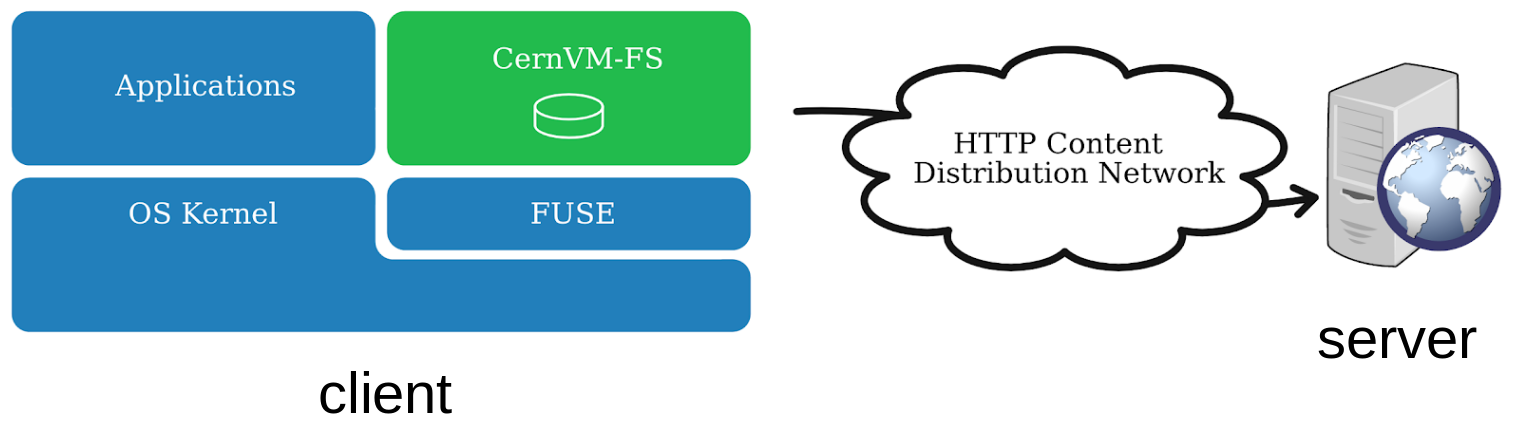
\includegraphics[scale=0.27]{figures/overview}
\par
By means of aggressive caching and reduction of latency, CernVM-FS focuses specifically on the software use case. Software usually comprises many small files that are frequently opened and read as a whole. Furthermore, the software use case includes frequent look-ups for files in multiple directories when search paths are examined.
\par
CernVM-FS is actively used by small and large HEP collaborations. In many cases, it replaces package managers and shared software areas on cluster file systems as means to distribute the software used to process experiment data.
\par
In contrast to general purpose network file systems such as NFS or AFS, CernVM-FS is particularly crafted for fast and scalable software distribution. Running and compiling software is a use case general purpose distributed file systems are not optimized for. In contrast to virtual machine images or Docker images, software installed in CernVM-FS does not need to be further packaged. Instead it is distributed and versioned file-by-file.

\begin{figure}[h]
\centering
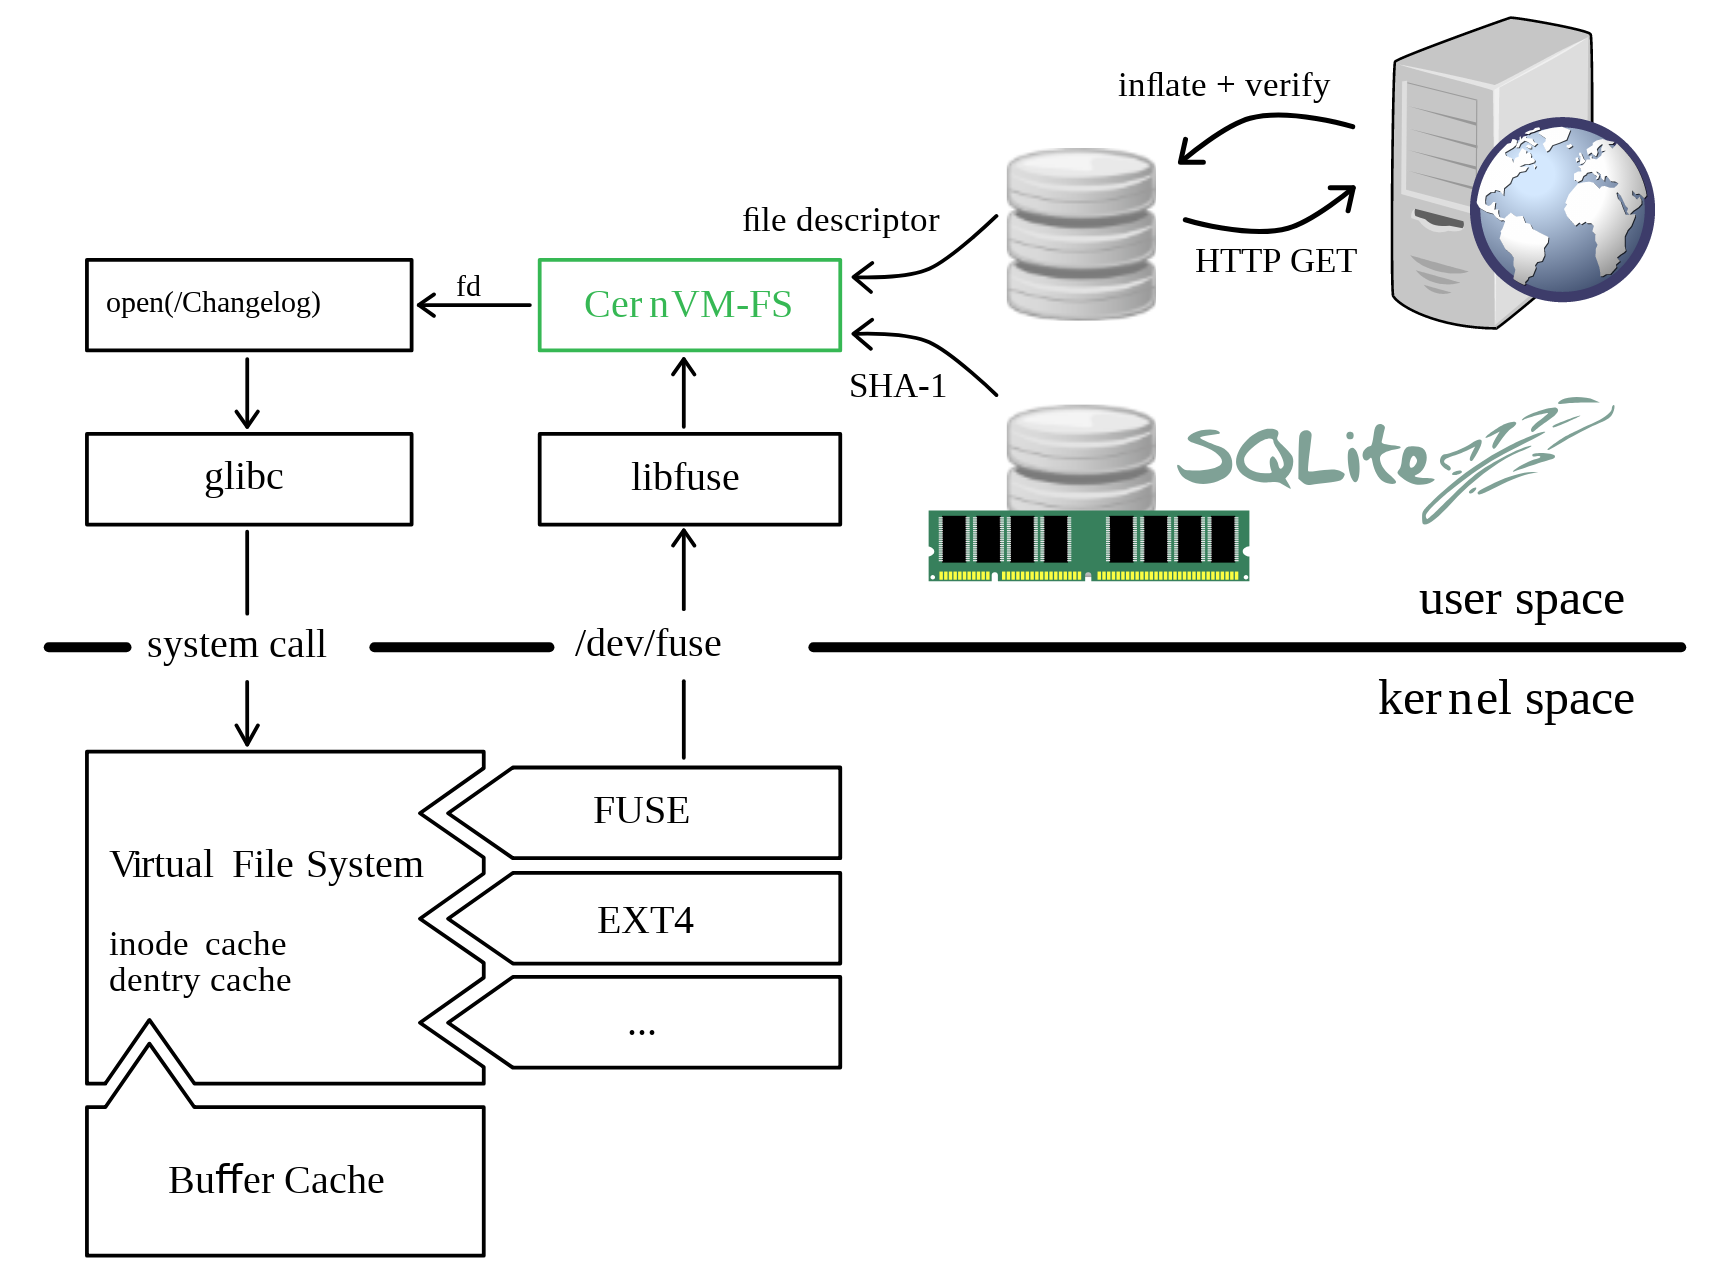
\includegraphics[scale=0.27]{figures/client_cvmfs}
\caption{\textit{On the client, only data and metadata of the software releases that are actually used are downloaded and cached.}}
\end{figure}
